\documentclass[shortpres]{beamer}
\usetheme{CambridgeUS}
\usepackage[utf8]{inputenc}

\setbeamertemplate{footline}
{
  \leavevmode%
  \hbox{%
  \begin{beamercolorbox}[wd=.333333\paperwidth,ht=2.25ex,dp=1ex,center]{author in head/foot}%
    \usebeamerfont{author in head/foot}\insertshortauthor%~~\beamer@ifempty{\insertshortinstitute}{}{(\insertshortinstitute)}
  \end{beamercolorbox}%
  \begin{beamercolorbox}[wd=.333333\paperwidth,ht=2.25ex,dp=1ex,center]{title in head/foot}%
    \usebeamerfont{title in head/foot}\insertshorttitle
  \end{beamercolorbox}%
  \begin{beamercolorbox}[wd=.333333\paperwidth,ht=2.25ex,dp=1ex,right]{date in head/foot}%
    \usebeamerfont{date in head/foot}\insertshortdate{}\hspace*{2em}
    \insertframenumber{} / \inserttotalframenumber\hspace*{2ex}
  \end{beamercolorbox}}%
  \vskip0pt%
}\part{title}
\beamertemplatenavigationsymbolsempty


%color specification---------------------------------------------------------------
\definecolor{TUMblue}{rgb}{0.00, 0.40, 0.74}
\definecolor{TUMgray}{rgb}{0.85, 0.85, 0.86}
\definecolor{TUMpantone285C}{rgb}{0.00, 0.45, 0.81}
\definecolor{lightblue}{rgb}{0.7529,0.8118,0.9333}

\setbeamercolor{block title}{fg=white, bg=TUMpantone285C}
\setbeamercolor{block body}{bg=lightblue}
\setbeamertemplate{blocks}[rounded][shadow=true]
%----------------------------------------------------------------------------------

\setbeamercolor{frametitle}{fg=TUMblue, bg=white}
\setbeamercolor{palette primary}{fg=TUMblue,bg=TUMgray}
\setbeamercolor{palette secondary}{use=palette primary,fg=TUMblue,bg=white}
\setbeamercolor{palette tertiary}{use=palette primary,fg=white, bg=TUMblue}
\setbeamercolor{palette quaternary}{use=palette primary,fg=white,bg=TUMpantone285C}


\setbeamercolor{title}{bg=white,fg=TUMblue}
\setbeamercolor{item projected}{use=item,fg=black,bg = lightblue}
\setbeamercolor{block title}{fg=black, bg=lightblue}
\setbeamercolor{block body}{bg=white}
\setbeamertemplate{blocks}[rounded][shadow=true]
%----------------------------------------------------------------------------------
\setcounter{figure}{0}


\usepackage{psfrag} %for \psfrag in figures
\usepackage{algorithm,algpseudocode}  %for algorithm environment
\usepackage{graphicx}

\title[Motion Planning for Autonomous Vehicles]{Clustering Similar Traffic Scenarios}

\author[]{Murat Can \"Uste, Zhaoying Chen, Qiaoxi Liu, Emanuel Ramneantu}
\institute[TU M\"unchen]{Technische Universit\"at M\"unchen}

\date{November 20, 2019}

\begin{document}

\begin{frame}
    \titlepage
\end{frame}


\section{Problem Statement}	

\begin{frame}{Problem of Testing Automated Vehicles}	

\begin{itemize} 
\item We need to test automated vehicles, but how?
\vfill \item  Can we cover all situations that occur in a traffic?
\vfill \item  Do we know all different situations that can occur, especially in microscopic level?
\end{itemize}
\end{frame}

\section{Proposed Method}	

\begin{frame}{Proposed Method}	

\begin{itemize} 
\item Cluster similar scenarios in order to group them based on their similarity, and test automated vehicle functions on a set of scenarios from each group to reduce testing and validation effort.
\vfill \item  Optional: Hierarchical clustering and automatic labeling of scenarios.
\end{itemize}

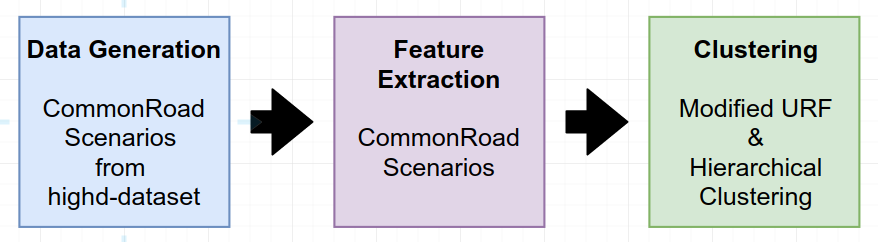
\includegraphics[width=\textwidth]{proposed_01}
\end{frame}

\section{Tasks}	

\begin{frame}{Tasks}	

\begin{itemize} 
\item Data generation
\vfill \item Feature extraction
\vfill \item Random Forest Clustering and Hierarchical Clustering
\end{itemize}
\end{frame}

\section{Data Generation}	

\begin{frame}{HighD Dataset}	

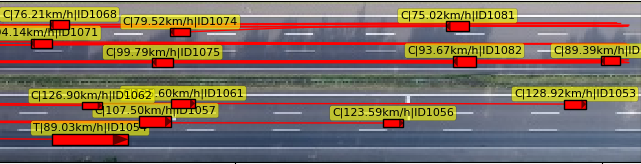
\includegraphics[width=\textwidth]{highd-example}

\begin{itemize} 
\item 60 recordings from 6 different highway locations, approx. 20 minutes per recording.
\vfill \item Information such as vehicle types, sizes, trajectories are already extracted. Also includes metrics such as TTC. DHW, THW, and lane changes.
\vfill \item Downside: There are no curvatures, intersections, static obtacles, or different types of dynamic obstacles such as pedestrians, bicycles etc.
\end{itemize}

\end{frame}


\section{Data Generation}	

\begin{frame}{HighD to CommonRoad Scenarios}	

\begin{itemize} 
\item Extract 2-3 sec. segments from raw data and convert them to CommonRoad Scenario format.
\vfill \item Extract based on minimum TTC for each vehicle (if they have), and set the minimum TTC frame as the middle point of the scenario.
\vfill \item The vehicle with the minimum TTC is selected as the ego vehicle, and it's trajectory is included as obstacle to the scenario for extracting features related to the ego vehicle.
\vfill \item About 10.000 scenarios. Multiplies if we also consider other vehicles as ego vehicle instead of the vehicle with the minimum TTC.
\end{itemize}

\vfill 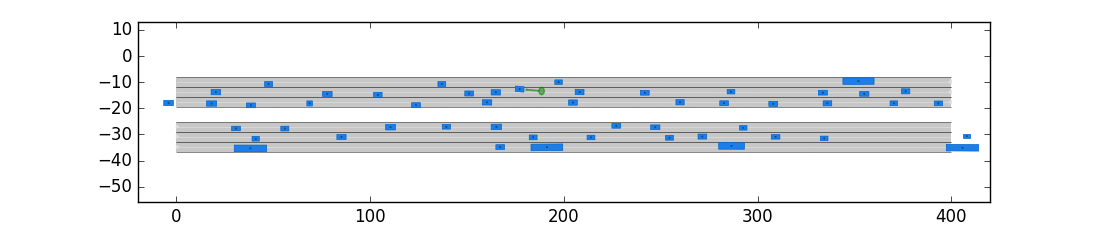
\includegraphics[width=\textwidth]{cr-example-15}

\end{frame}

\section{Feature Extraction}	

\begin{frame}{Feature Extraction}	

\begin{itemize} 
\item Why feature extraction: to build a quantitative model for the scenario
\vfill \item The goal of feature extraction: to give an approximate balance to capture the characteristics of scenarios, while being compact for fast computation
\vfill \item Model
\vfill \item Example
\end{itemize}
\end{frame}

\section{Feature Extraction}

\begin{frame}{Scenario Model}
    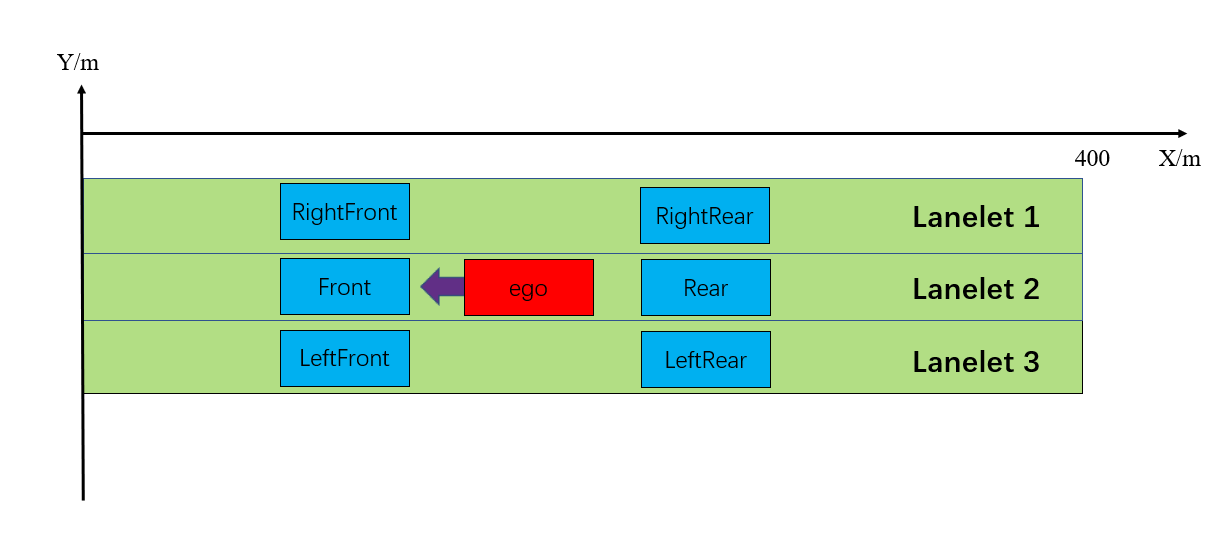
\includegraphics[height=0.6\textheight]{ScenarioModel.png}
\end{frame}

\section{Feature Extraction}

\begin{frame}{Feature Structure}
    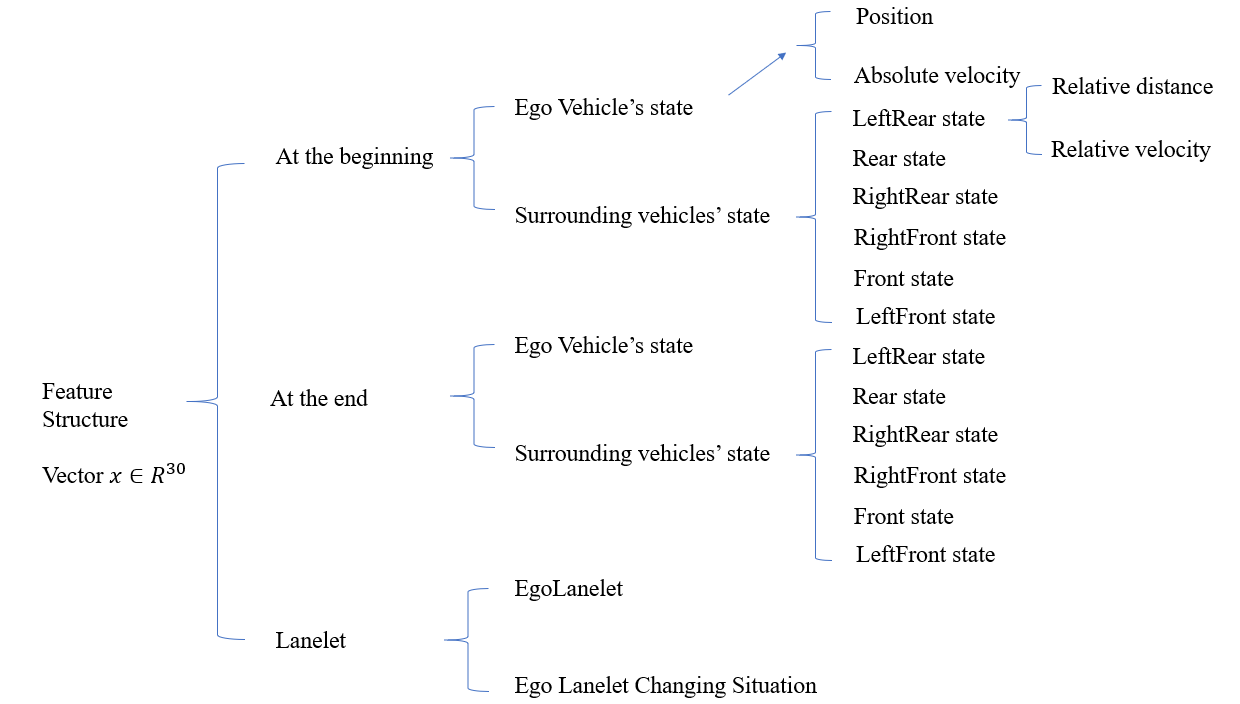
\includegraphics[width=12cm,height=6.5cm]{Feature_Structure.png}
\end{frame}

\section{Feature Extraction}

\begin{frame}{Example}
    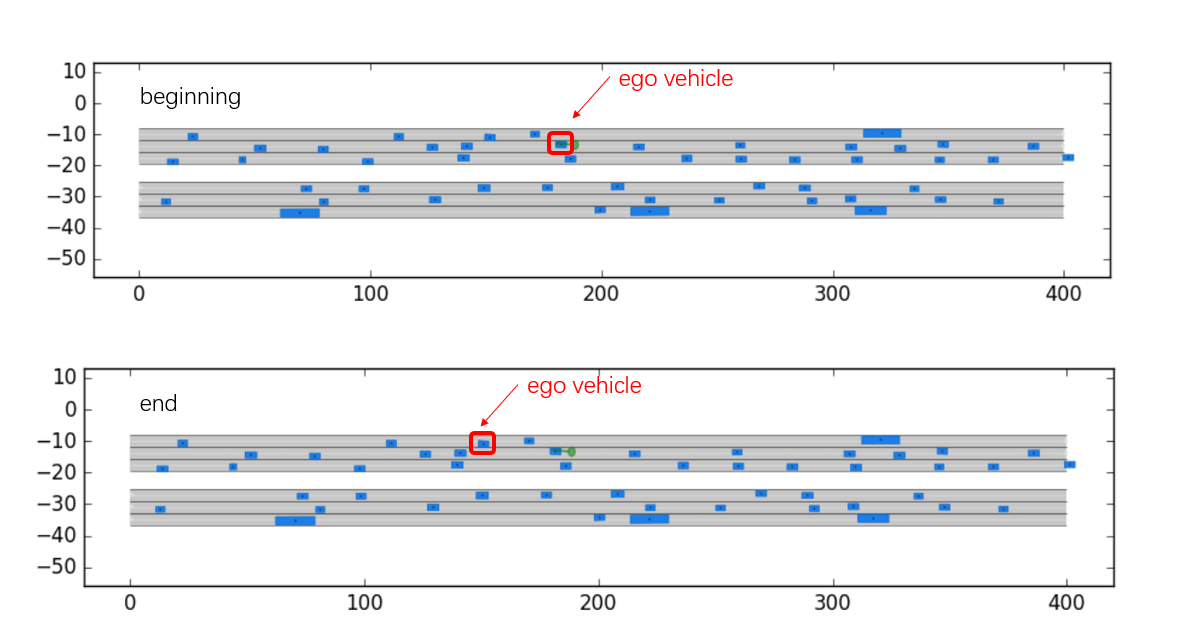
\includegraphics[width=12cm,height=6cm]{LaneletChangingExample.png}
\end{frame}

\section{Feature Extraction}
\begin{frame}{Example}
    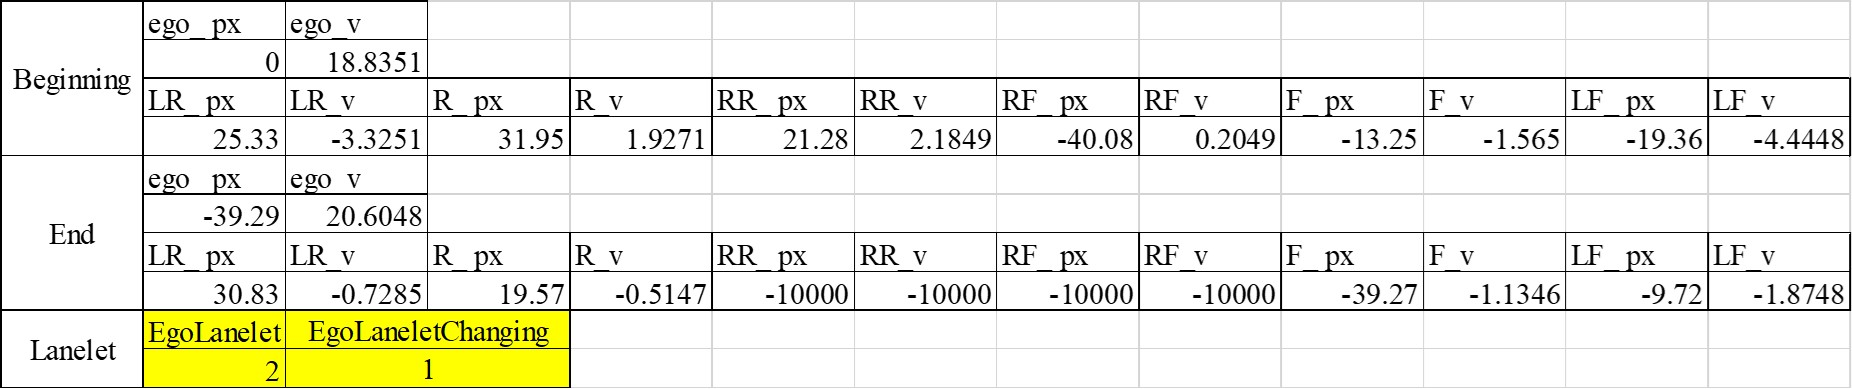
\includegraphics[width=12cm,height=3cm]{FeatureTable.jpg}
\end{frame}

\section{Clustering}	

\begin{frame}{Clustering}	

\begin{itemize} 
\item Random forest
\begin{itemize}
\item A collection of random trees used for classification
\item Generate synthetic points
\item Use organic/synthetic as response variable
\end{itemize}
\item Proximity matrix
\begin{itemize}
\item Multiple ways to generate (Leafs, Paths)
\item Multiple clustering algorithms (PAM, Hierarchical)
\end{itemize}
\item Visualization
\begin{itemize}
\item Heatmap, dendrogram $\rightarrow$ not much insight
\item Parallel/sequential playback
\end{itemize}
\end{itemize}
\end{frame}
\begin{frame}{Ensemble Learning: Random Forest}	
  \begin{itemize} 
    \item Good estimator of the feature importance 
    \item Intuitive and easy to implement
    \item Reducing overfitting
  \end{itemize}
  \begin{figure}
    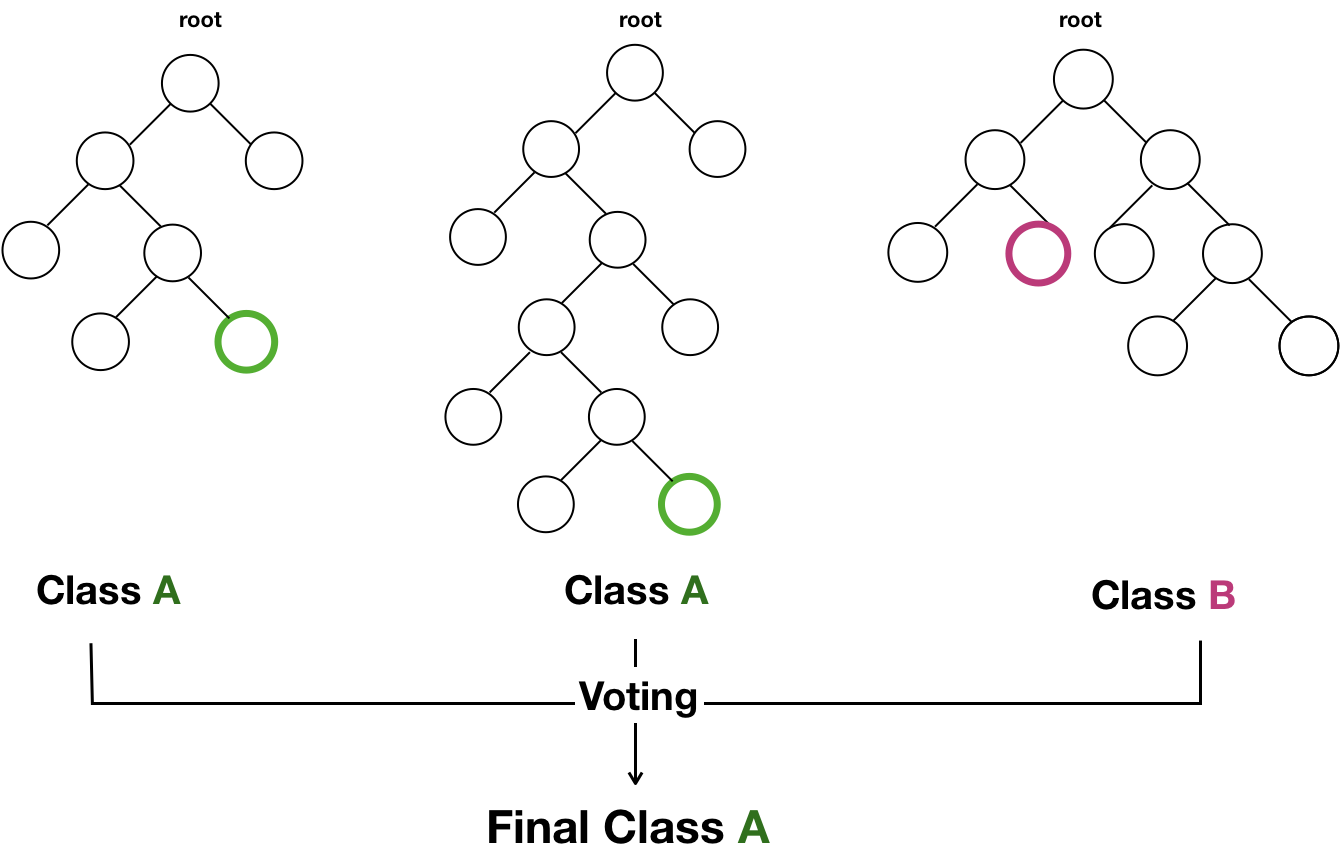
\includegraphics[height=0.6\textheight]{fig/forest0.png}
  \end{figure}
\end{frame}
\begin{frame}{Training on Nomal Decision Tree (DT)}	
  \textbf{With labels} A,B,C,D,  Get classification result and corresponding split features
  \begin{figure}
    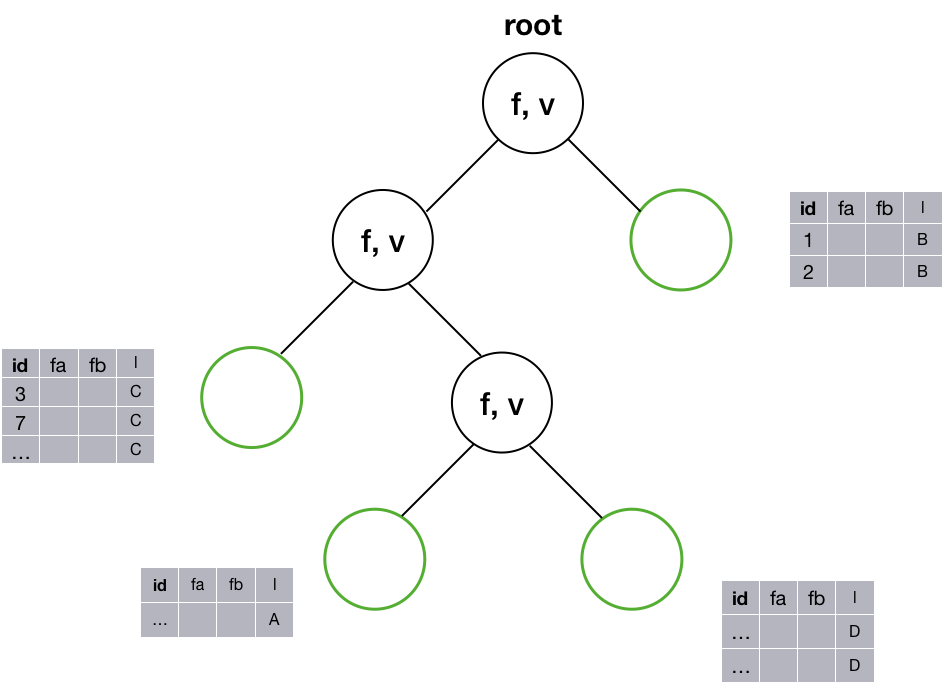
\includegraphics[height=0.6\textheight]{fig/dt3.png} 
  \end{figure}
  \end{frame}
\begin{frame}{Challange for Clustering}	
\textbf{Without labels..?} 

  \begin{figure}
    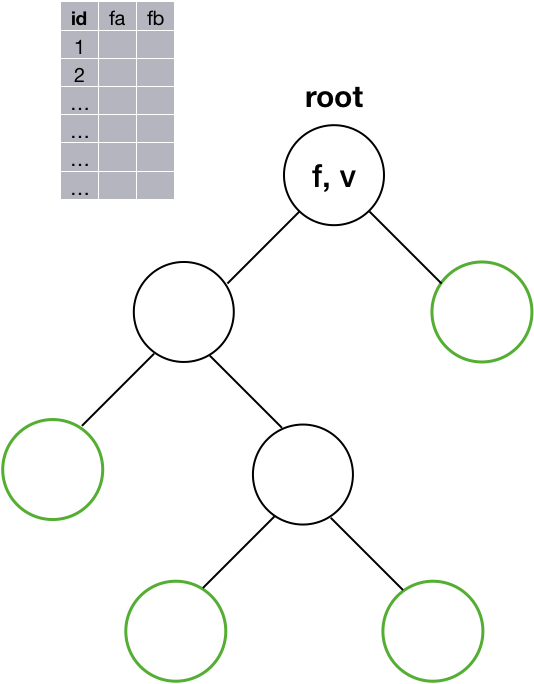
\includegraphics[height=0.6\textheight]{fig/dtwithout1.png} 
  \end{figure}
  \end{frame}
  \begin{frame}{Initial Solution}	
    \textbf{Without labels...!} 
    \begin{itemize} 
      \item Adding same label (e.g. 0) for orginial data $(\mathcal{D})$ and generate synthetic data $(\mathcal{S})$ labeled with 1
      \item Training them together as normal DT
    \end{itemize}
      \begin{figure}
        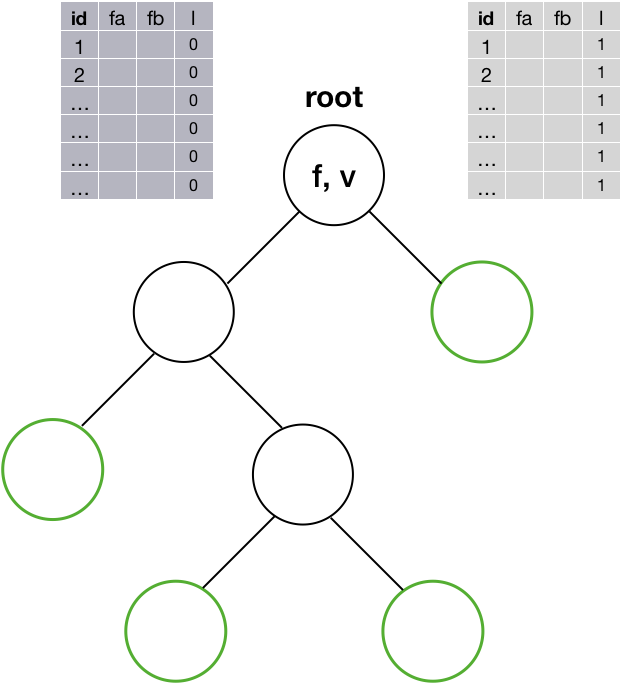
\includegraphics[height=0.5\textheight]{fig/dtwithout3.png} 
      \end{figure}
      \end{frame}
      \begin{frame}{Drawback of Initial Solution}	
        \begin{itemize} 
          \item high dimensional input $\rightarrow$ no more $\mathcal{S}$ left $\rightarrow$ large leaves
          \item large amount of $\mathcal{S}$ $\rightarrow$ unbalanced ratio between $\mathcal{S}$ and $\mathcal{D}$
        \end{itemize}
          \begin{figure}
            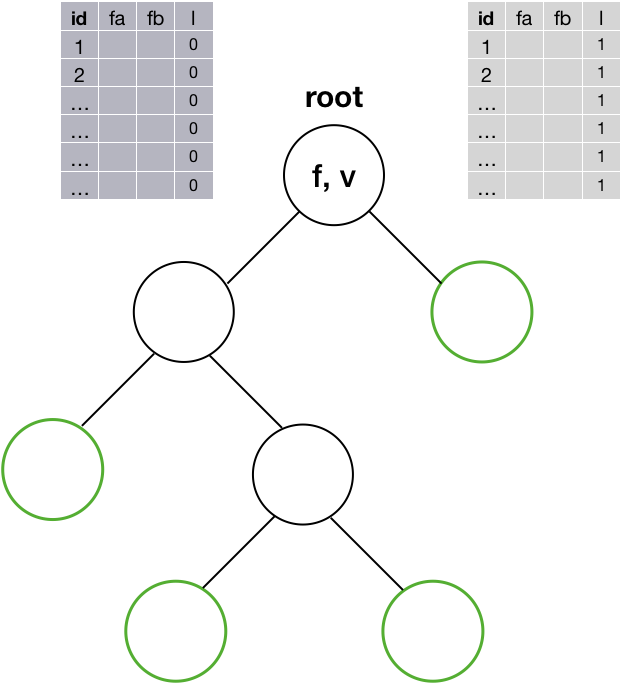
\includegraphics[height=0.5\textheight]{fig/dtwithout3.png} 
          \end{figure}
          \end{frame}
  \begin{frame}{A Better Solution: CLustering Tree}	
    \begin{itemize} 
      \item For each split: Add equal number of data from $\mathcal{D}$ in that node.
      \item Training them together as normal DT
    \end{itemize}
    \begin{figure}
      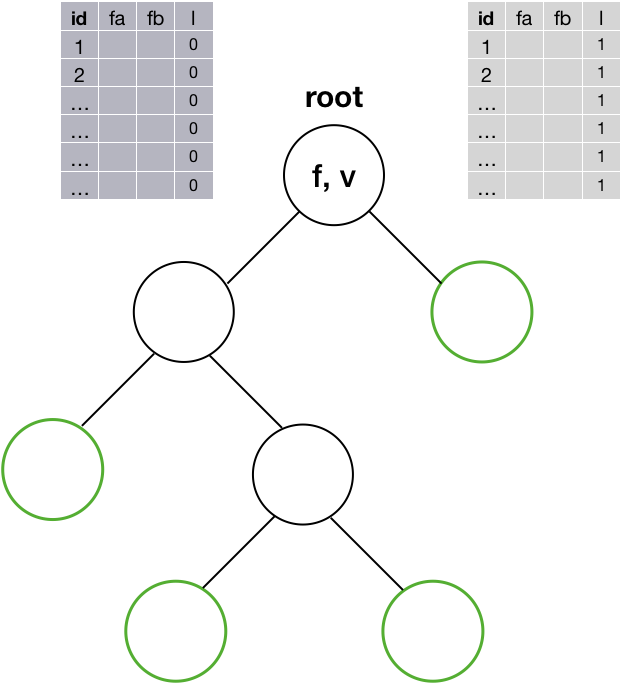
\includegraphics[height=0.6\textheight]{fig/dtwithout3.png} 
    \end{figure}
    \end{frame}
  \begin{frame}{Details for CLustering Tree}	
    At each split, we:
    \begin{itemize} 
      \item generate a uniformly distributed data (for each dimension) points
      \item put them with original data together to compute the "best" feauture as well as the splitting value based on gini-impurity.
    \end{itemize}   
    \begin{figure}
      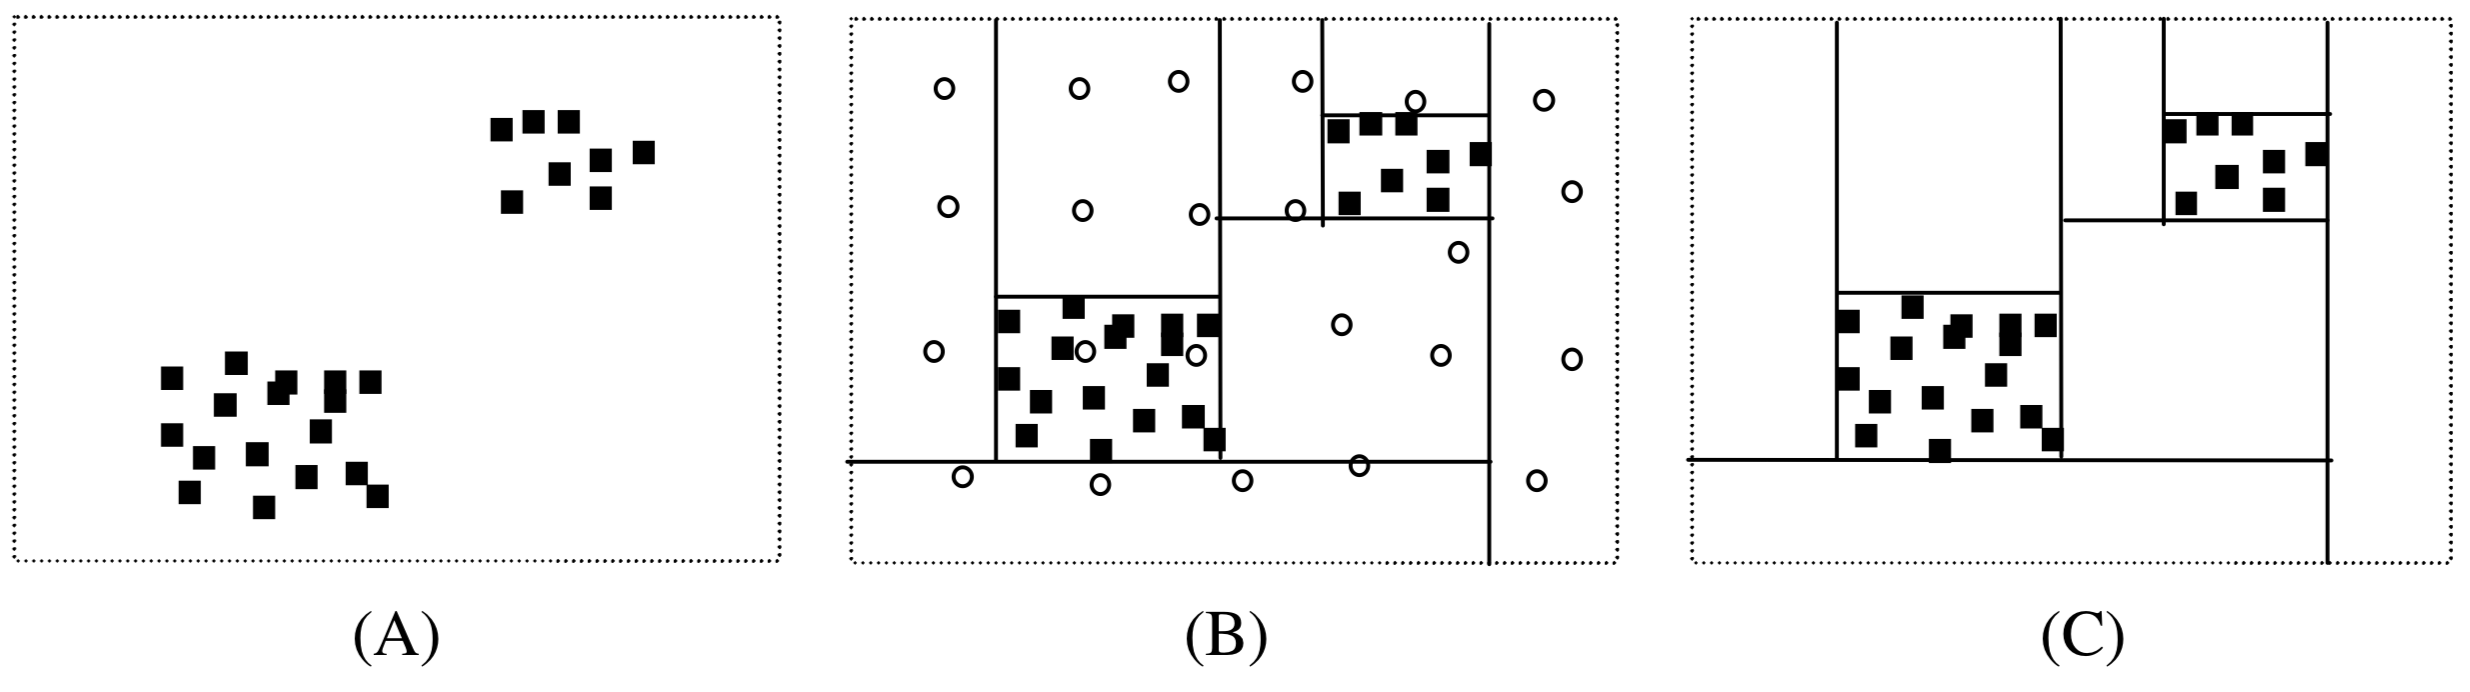
\includegraphics[width=0.8\textwidth]{fig/random_noise_clustering.png}
    \end{figure}
  \end{frame}
  \begin{frame}{Demo of Creating a Clustering Tree}	
    \begin{figure}
      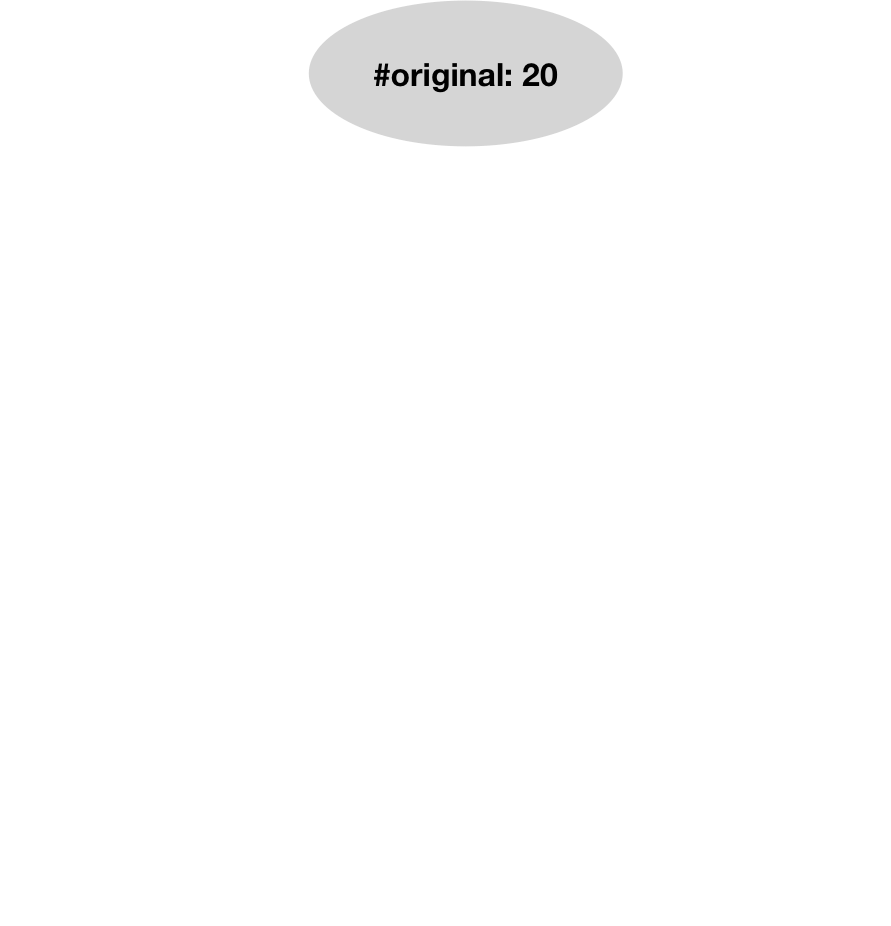
\includegraphics[height=0.6\textheight]{fig/cltree.png}
    \end{figure}
  \end{frame}
  \begin{frame}{Demo of Creating a Clustering Tree}	
    \begin{figure}
      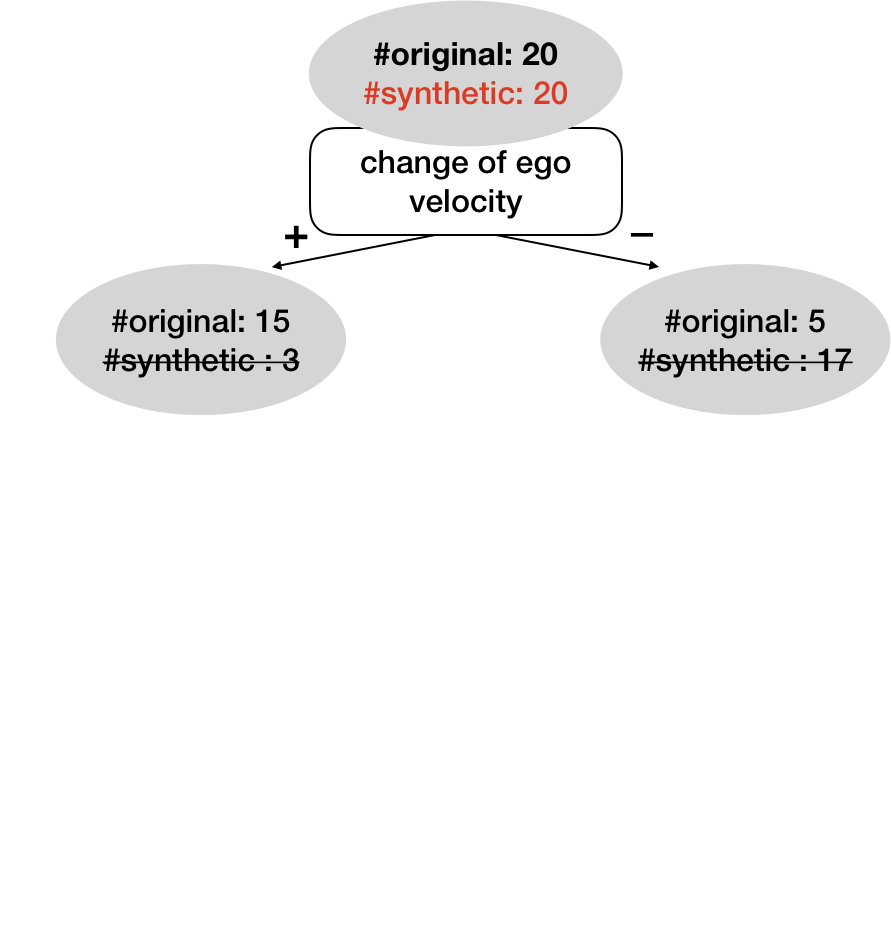
\includegraphics[height=0.6\textheight]{fig/cltree1.png}
    \end{figure}
  \end{frame}
  \begin{frame}{Demo of Creating a Clustering Tree}	
    \begin{figure}
      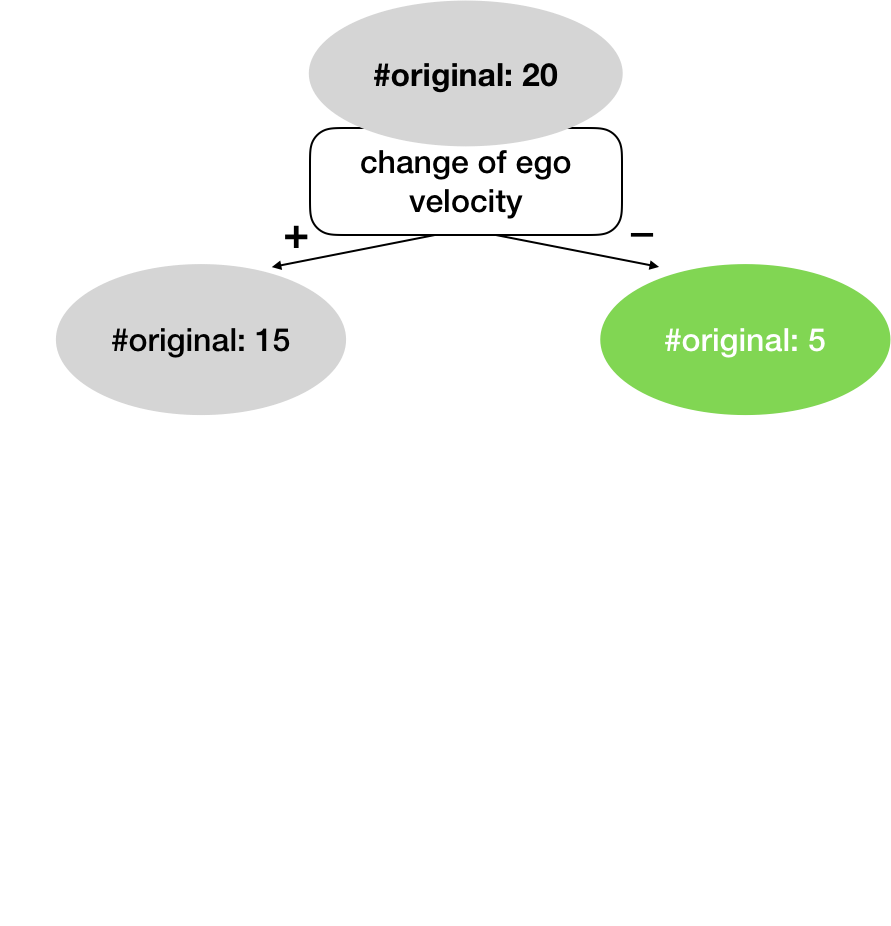
\includegraphics[height=0.6\textheight]{fig/cltree2.png}
    \end{figure}
  \end{frame}
  \begin{frame}{Demo of Creating a Clustering Tree}	
    \begin{figure}
      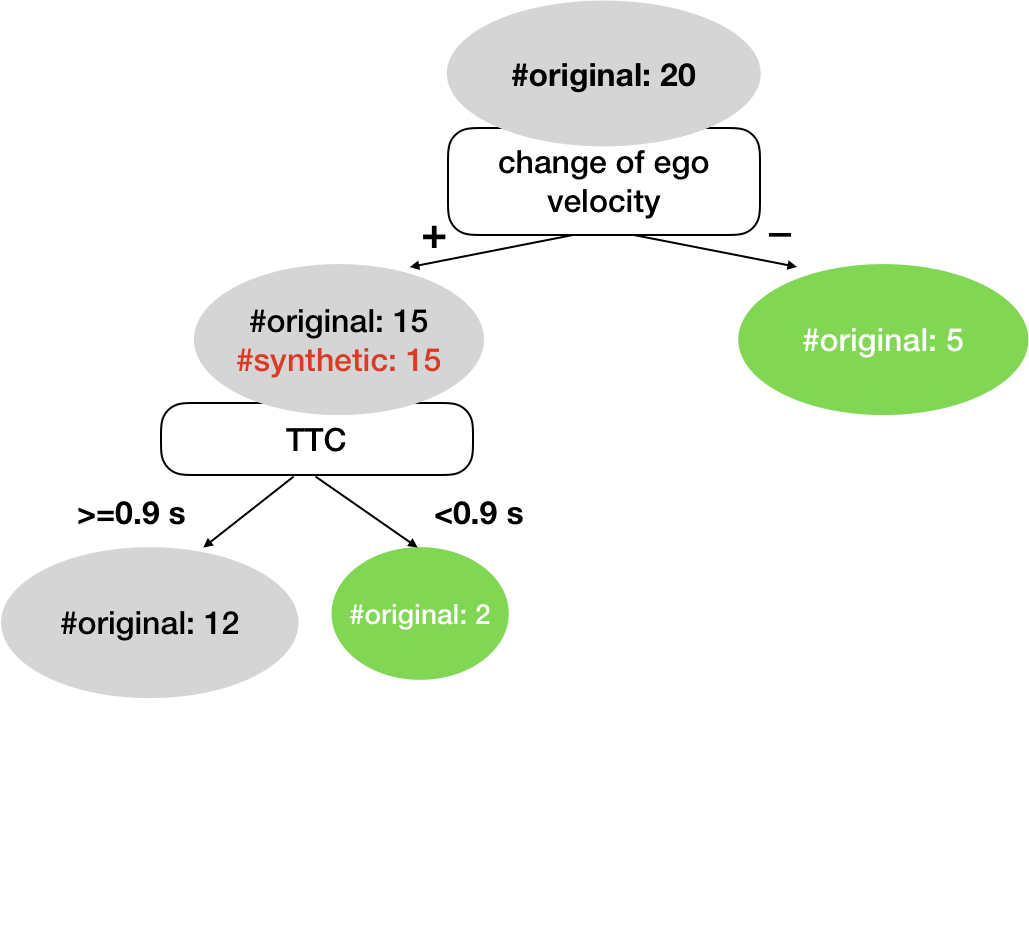
\includegraphics[height=0.6\textheight]{fig/cltree3.png}
    \end{figure}
  \end{frame}
  \begin{frame}{Demo of Creating a Clustering Tree}	
    \begin{figure}
      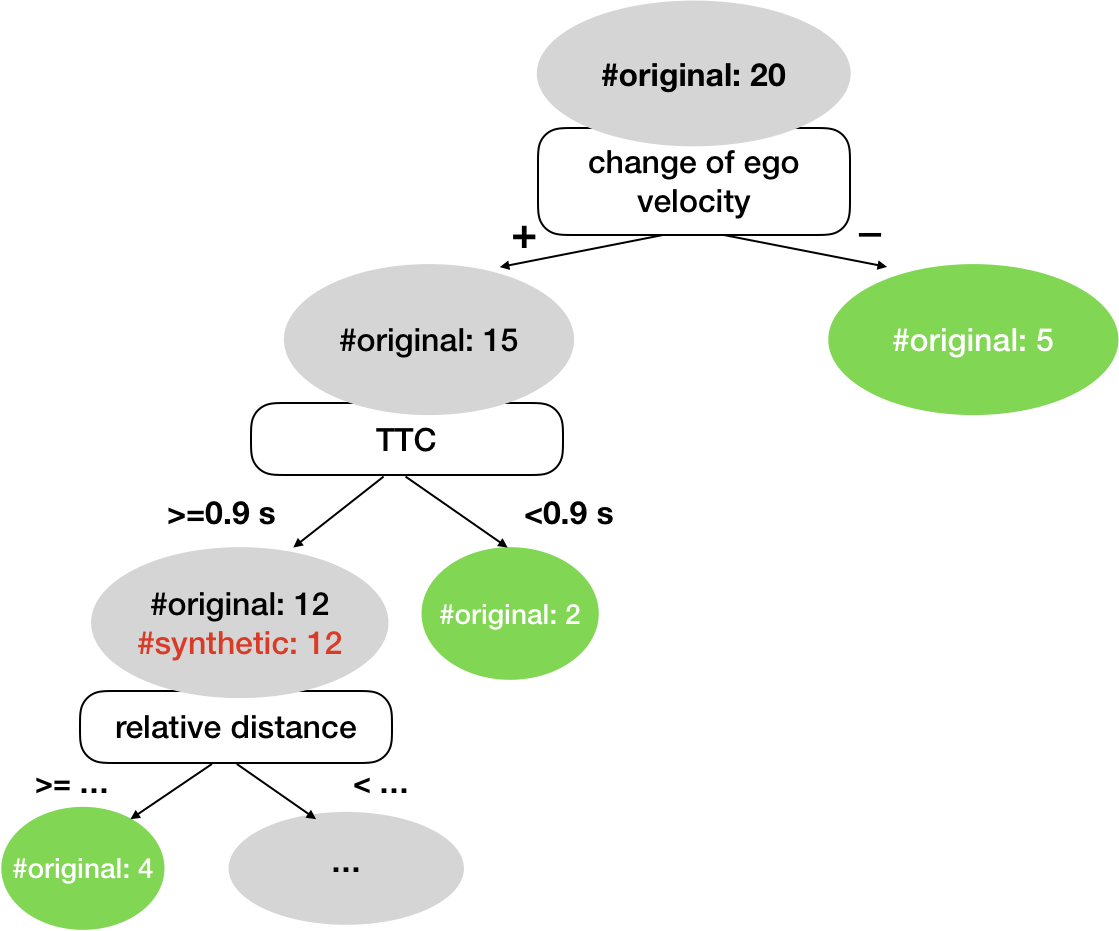
\includegraphics[height=0.6\textheight]{fig/cltree4.png}
    \end{figure}
  \end{frame}
  \begin{frame}{Proximity Path}	
    For one tree T, the path of scenario i (as a part of one leaf) defined as a set $T_i$ including all nodes the i passed.
    $$T_i = \{t_1,...,t_n\}$$
    \begin{figure}
      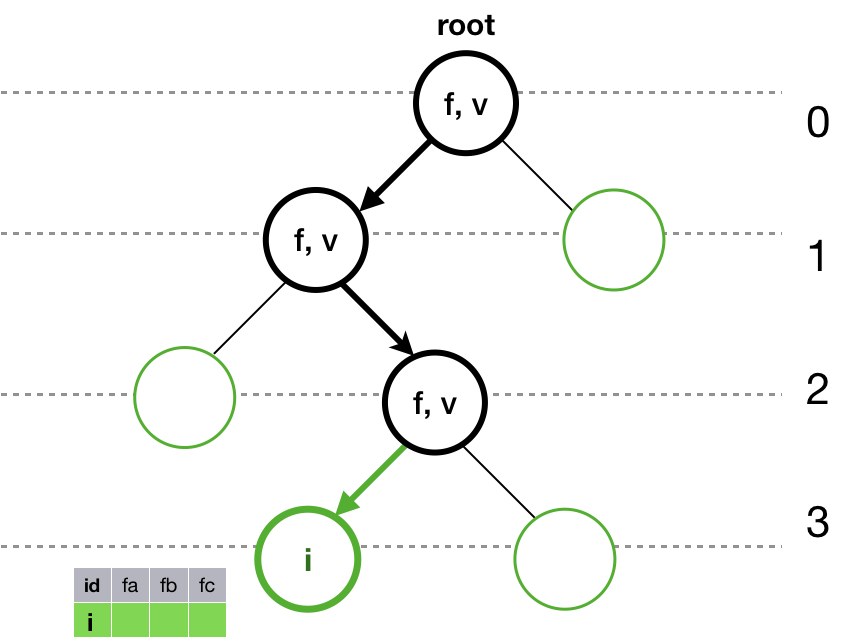
\includegraphics[height=0.6\textheight]{fig/ppath.png}
    \end{figure}
  \end{frame}
  \begin{frame}{Proximity Path}	
    Intersection: $|T_i \cap T_j|$; Difference: $|T_i|+ |T_j|-|T_i \cap T_j|$
    \begin{figure}
      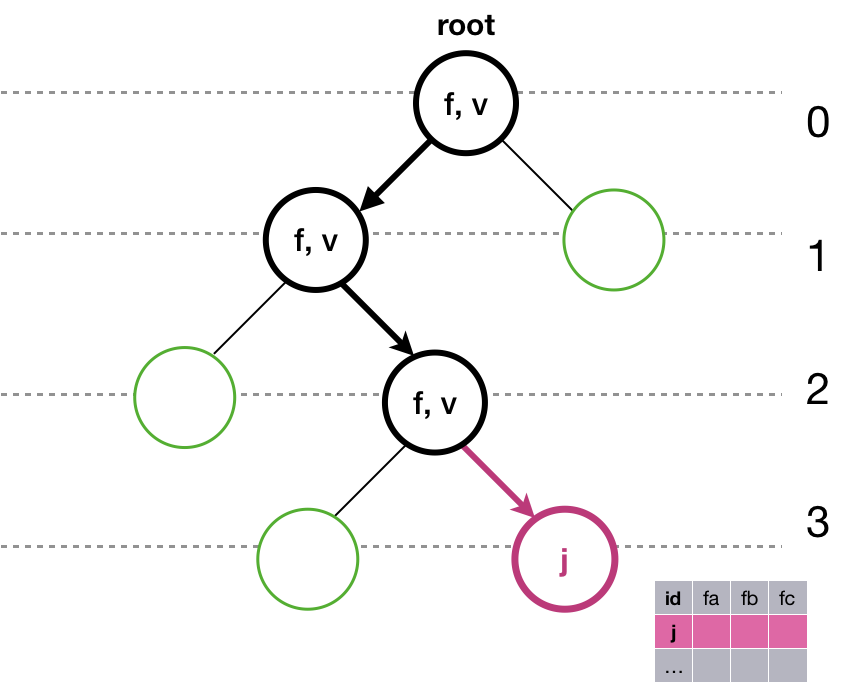
\includegraphics[height=0.6\textheight]{fig/ppath2.png}
    \end{figure}
  \end{frame}
  \begin{frame}{Proximity Path}	
  the Proximity (Jaccard Index) between i,j is:

  $$P_{ij}=\frac{|T_i \cap T_j|}{|T_i \cup T_j|} \in (0,1]$$ 0: no mutual path; 1: exactly same path
    \begin{figure}
      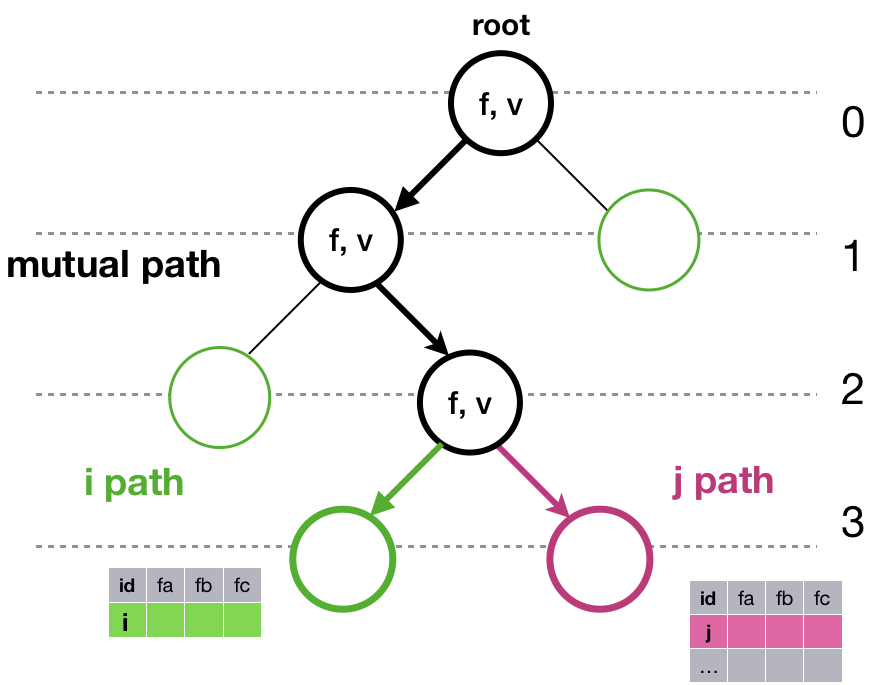
\includegraphics[height=0.5\textheight]{fig/ppath3.png}
    \end{figure}
  \end{frame}






\begin{frame}{Hierarchical Clustering}

\begin{columns}
\begin{column}{0.6\textwidth}
\begin{itemize}
\item \textbf{Goal:} Given a proximity matrix, compute clusters
\item \textbf{Procedure:} Sequentially group similar data points together
\item Questions:
\begin{itemize}
\item When to stop
\item How to compute distance between clusters
\item How to reorder leafs
\end{itemize}
\end{itemize}
\end{column}
\begin{column}{0.4\textwidth}
\begin{figure}[h!]
	\vspace{-1em}
  \centering
    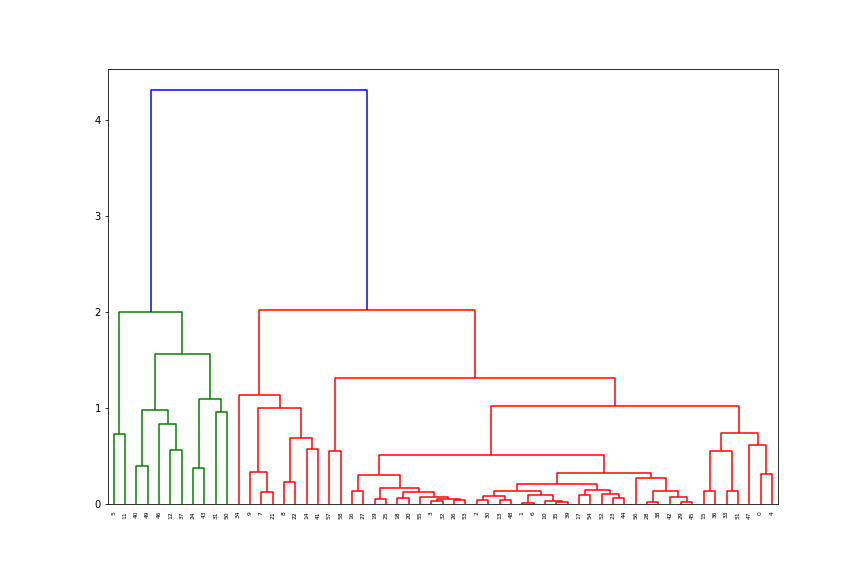
\includegraphics[width=\textwidth]{dendro.png}
  \vspace{-2em}
  \caption{Dendrogram}
\end{figure}
\end{column}
\end{columns}

\end{frame}

\begin{frame}{Proximity matrix}
\begin{columns}
\begin{column}{0.5\textwidth}
\begin{figure}[h!]
  \centering
    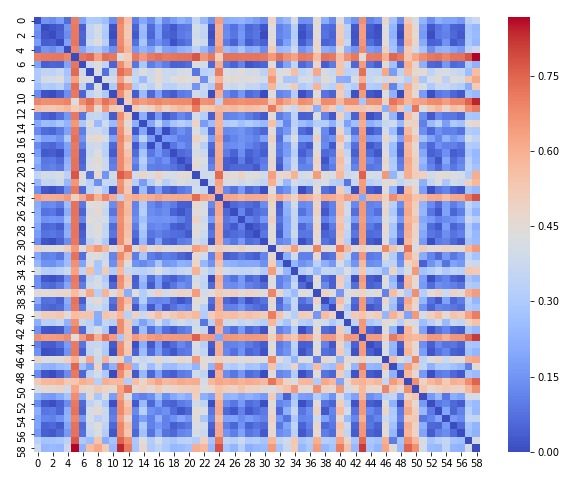
\includegraphics[width=\textwidth]{heatmap.png}
  \caption{Distance matrix}
\end{figure}
\end{column}
\begin{column}{0.5\textwidth}
\begin{figure}[h!]
	\vspace{-1em}
  \centering
    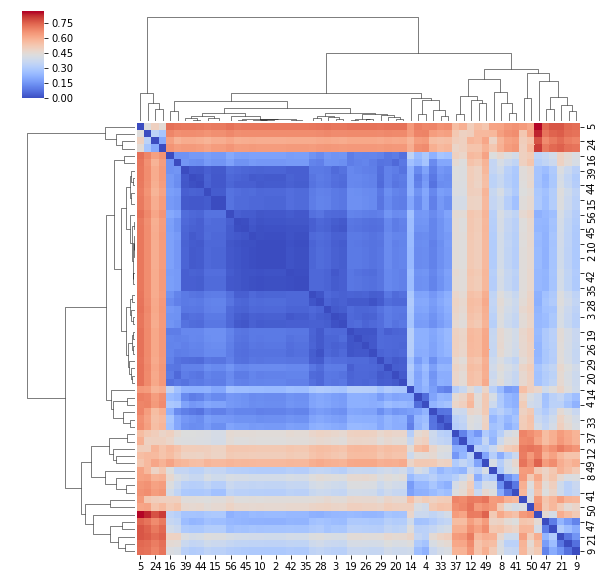
\includegraphics[width=\textwidth]{map.png}
  \vspace{-2em}
  \caption{Sorted heatmap matrix}
\end{figure}
\end{column}
\end{columns}
\end{frame}

\begin{frame}{Causes for similarity}

Calculate correlation between clusters and features

\begin{figure}[h!]
  \centering
    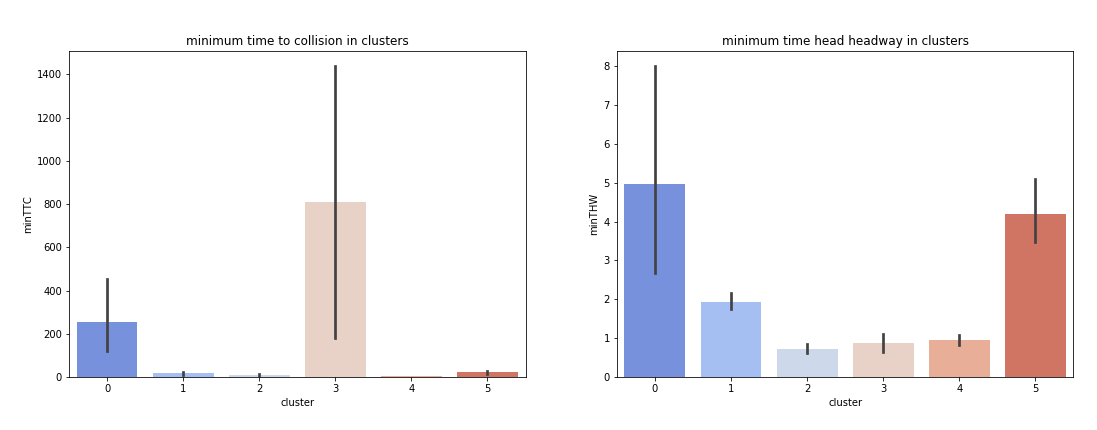
\includegraphics[width=\textwidth]{clusters.png}
  \vspace{-2.4em}
  \caption{Feature plots}
\end{figure}

\end{frame}

\section{Challanges}	

\begin{frame}{Challanges Related to the Implementation}	

\begin{itemize} 
\item Data set is limited, so we can't get wide variety of scenarios.
\vfill \item Hard to filter out redundant situations which will not be interesting enough for the motion planning algorithms, such as empty straight road.
\vfill \item Feature extraction: strike a balance between describing the scenario more detailed and using less features.
\vfill \item  How many clusters to choose. (setting of minimum number of datapoints within a cluster, etc.)
\vfill \item  How to evaluate our final clustering results. 
\end{itemize}
\end{frame}

\section{Timetable}	

\begin{frame}{Timetable and Milestones}	

\begin{itemize} 
\item \textbf{Week 1}, 14.10.2019 - 20.10.2019: Introduction lecture and software tutorial.
\vfill \item  \textbf{Week 2 \& 3}, 21.10.2019 - 03.11.2019: Team Meatings and Literature review
\vfill \item  \textbf{Week 4 \& 5}, 04.11.2019 - 17.11.2019: Initial implementation of the tasks and preparation for the concept presentation.
\vfill \item  \textbf{Week 6 \& 7}, 18.11.2019 - 01.12.2019: First Iteration - Full implementation with simple features
\vfill \item  \textbf{Week 8 \& 9}, 02.12.2019 - 15.12.2019: Review and Refinement
\vfill \item  \textbf{Week 10 \& 11}, 16.12.2019 - 12.01.2020: Second Iteration - Full implementation with more/refined features.
\vfill \item  \textbf{Week 12 to 14}, 13.01.2020 - 02.02.2020: Writing report and preparing for the final presentation.
\end{itemize}

\end{frame}

\end{document}
